\chapter{Party Hard}

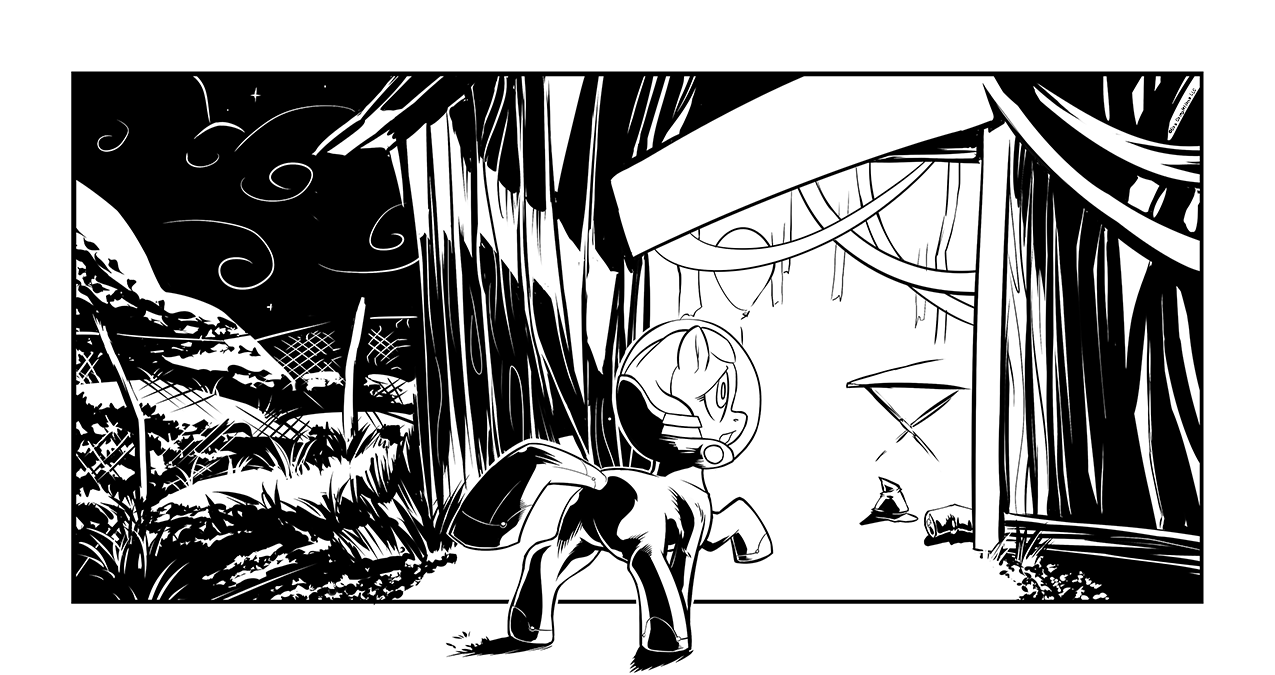
\includegraphics[width=0.9\linewidth]{image02.png}

\begin{intro}
No need to bring a gift, being there will be enough!
\end{intro}

\englishdaytimeplace{2}{4:00 P.M.}{Redtrotters Ridges, Big 52, N. Branch}

Usually, wearing a full environmental suit is not considered the cutting edge of Equestrian fashion, but anypony has to admit that it brings some neat advantages. First of all, if you were to survive a direct hit from a balefire bomb, you'd probably live long enough to die of thirst inside the suit before the radiation got you. The other good thing about being inside a hermetically sealed, radiation shielded suit is you'll never want for an umbrella or sunscreen again. And being lemon yellow, it's nearly impossible to go anywhere unnoticed unless, perhaps, you've been buried under an avalanche of lemons. Obviously there are moments in the Wasteland where stealth is a virtue.

As if Puppy even knew the meaning of the word.


\horizonline


"Hi! I'm Puppysmiles!" She beamed at the two new ponies in front of her. Their uniforms, if they could be called that, resembled the trio from the other night's, but seemed cleaner and less ragged. One, a unicorn mare, scanned the road behind Puppy with her caravan shotgun, searching for what was to her an obvious ambush. Beside her, her earth pony partner kept a large spear levelled at Puppy. Had the foal been a wiser pony, the two mare's actions might have worried her.

The unicorn was the first to talk. "What are you doing in Redtrotter territory, foal?"

"And what the hay is that weird suit?" added the earth pony.

"I'm looking for my mom!" Puppy replied enthusiastically, pointing a hoof more or less in the direction the road was going. "She's that way!"

The two tribe ponies exchanged a glance before the unicorn spoke again. "Okay, and what's your mother's name? Is she a Redtrotter?"

"What's a Redtrotter?"

The unicorn, her unease flaring into anger, prepared to go ballistic on Puppy. Sensing this, her partner stepped in. "We are the Redtrotters. We control the Transequestrian Route 52 from here to Salt Cube City. If you have business on the Big 52 you do it through us. So, what's your mother's name?"

``My mommy is called Rainy Days! She's super cool and she always sings for me and she's a great cook too! She's the best pony ever and when I'm big I want to be like her!''

``Yeah, all right kid, I get the point,'' snapped the unicorn. ``I don't know a Rainy Days, so she's definitely not a Redtrotter. Are you alone? Who sent you here?''

``Mister Voice is with me!''

``Mister Voice?'' The unicorn warily surveyed the road again.

``Yeah! He lives in my space suit and sometimes we sing together but sometimes he gets grumpy but it's okay because he's helping me find Mom!''

\emph{``Right.''} The mare lowered her guard. ``Look, I'm sorry, but if you and your invisible friend want to pass through here, you need to pay the fee.''

``Ah, okie dokie? I have\dots'' Puppy started searching the many pockets of her suit. She had amassed a small hoard of junk in her short travel, mostly broken toys and things she thought were interesting. Maybe she had something these ponies would like. After all, \emph{you gotta share, you gotta care,} right?  ``What about this?''

Manipulating things without her teeth was quite a problem. She had to use her hooves instead. This task was only made more difficult by her bulky rubber boots, and the fact that she had to bend her leg at an awkward angle in order to reach into her saddlebags. ``Just a minute, I've almost got---no, uh.''

{\mt ``Assistance. The suit is equipped with a weak manipulation spell. Access your Inventory from the HUD and ask for the required item.''}

``Wut?''

The earth pony watched as Puppy mumbled to herself while fumbling out various useless junk from her saddlebags. The filly obviously couldn't pay. The spearmare looked at her friend and caught a meaningful glance. She sighed wistfully and after a brief internal prayer to the cruel gods of fate, plunged her spear into the foal's neck. Puppysmiles was so busy listening to the suit that she never saw it coming. She dropped to the ground like a sack of bricks, the earth pony letting her fall, silently cursing the Wasteland.

``You did her a favor. She wouldn't have lasted a day without her mother, and we can't afford to take her in. Better that we made it quick then let her get eaten by a manticore, or worse. You know what happens to foals around here,'' the unicorn trailed off with a sigh.

The earth pony noticed the troubled expression of her companion. ``Yeah. Poor Ridge Racer.''

The spearmare retrieved her weapon from the body. As she stepped back, pink smoke began to escape from the hole in the suit. The mare stared at the phenomenon, puzzled. ``Hey, Boney, what's that?''

The unicorn scratched her head with a hoof. ``You must have broken some talisman in the suit. It could be poisonous. Best to stay back.''

``We can't just leave her here, it doesn't feel right.'' The earth pony hesitated, trying to keep away from the pink smoke.

``After that funky little smoke show, I'm not going near her! The radroaches can take care of it. Come on, we still have a patrol to finish.''

With a final look at the fallen foal, the two mares trotted away, leaving the main road before climbing over a low ridge and out of sight. Time passed as the body of the filly in yellow lay alone in the middle of the road. A cold breeze picked up, rustling the bare trees. Despite the wind, the pink cloud that surrounded her did not seem to dissipate.


\horizonline

\englishdaytimeplace{2}{4:30 P.M.}{Redtrotters Ridges, Big 52, N. Branch}

The first sign that the lance had failed in its purpose was the automated speech of the suit coming back to life with a series crackles.

{\mt ``Initializing system. Checking version. Warning. Version number not corresponding. Starting in emergency mode. Version 0.2. Checking equipment status. All systems online. Major breach detected. Repair spells activated. Resuming last session. Loading personal data for subject 001: Puppysmiles. Subject deceased, condition stable. All clear.''}

Puppy's eyes began to blink for a moment inside the helmet, as if she had just awoken from a pleasant sleep. The foal yawned and a droplet of pink, glittering fluid fell from her mouth and onto the helmet of the suit, disappearing almost immediately as it was absorbed by the glass.

``Uhm, five more minutes, Mom.'' She turned around, still surrounded by the pink cloud that was now slowly fading.

{\mt ``Breach repaired. Subject insulated from external environment.''}

Lazily, Puppy got up and looked around. She frowned at the unfamiliar settings for a few moments before her memories came flooding back. ``Oh, right, Mom's not here. What was I doing before going to sleep?'' Puppy tried to scratch her head, but her hoof found the helmet on its way. She frowned again, then shrugged and continued to scratch the helmet thoughtfully.

{\mt ``Retrieving temporary memory. Query: last performed action before losing senses---negotiating passage.''}

``Negotiating what?''

{\mt ``Interacting with self-proclaimed Redtrotter ponies.''}

Fancy words again. ``Red-who?''

{\mt ``Talking with the pretty ponies.''}

At last, something comprehensible! ``Oh, right, pretty ponies! Now I remember! Ah, where have they gone?''

{\mt ``Location of Redtrotters unknown. Adding `Find the Redtrotter's' to the active mission list.''}

Puppy raised an eyebrow with a stumped expression. ``We have a to-do list? Since when?''

{\mt ``List initiated 23 hours ago. Objectives on the list: four.''}

``Wow, we have a lot of things to do! Four is a lot, right? What's on the list?''

{\mt ``Main objective: Reach MoM. Secondary objective: Get rid of space suit. Secondary objective: Confront Count Horse Tile or continue avoiding him. Secondary objective: Find the Redtrotters.''}

After listening to the list, the filly in yellow tapped her helmet with a hoof, a thoughtful expression on her muzzle. ``Think, think think. Muffins! No wait, that wasn't it.'' 

After several minutes of thinking, the foal finally nodded, a new resolve shining in her eyes. ``Okie dokie, play some music. Ah, the one with the chatty pony.'' Puppy trotted along the road, following the arrow and listening to the radio with a spring in her step.

The area surrounding Route 52 was a scorched wasteland dotted with rocks and ridges. It was hard to see very far because of the irregularity of the terrain. This normally would have been a problem, had Puppy any sense about her.

``Hey, Mister Voice, did you say something about taking stuff from my pockets?''

{\mt ``Affirmative. This suit is equipped with a weak manipulation spell.''}

``Uh, how does it work?''

{\mt ``Loading instructions. Selecting easy version for foals and Derpy. Name the object you need. If it is in your possession it will be put in front of you.''}

``Ah, muffins!'' A box of two hundred year old muffins floated in front of Puppy. She giggled. It looked so silly hovering in the air like that! ``Hey, this is fun! Sarsaparilla!'' A bottle of sarsaparilla replaced the muffins. ``Toy cart!'' This time a small toy cart in poor condition floated in front of the foal. ``Tee-hee! We need more stuff, I like this guessing game!''

{\mt ``Negative. This is not a guessing game. It is inventory management.''}

Puppy took a rock and put it in her pocket. ``A rock!'' The rock floated out of the pocket and listed lazily in front of her. ``Yay! It works!'' When it was put away again, the stone was labeled \emph{The Rock Of Destiny}, but since Puppy was not so good with reading, she didn't notice.

Trotting down the road, the filly kept asking for everything she had in her backpack, which really wasn't very much. She only owned four objects, but she planned on changing that soon. ``Oh, and we need more music!''

\begin{music}
		I can see that lone star from a thousand miles away
	
		Calling me back home, though I ventured far astray.
	
		When I see that beacon shining for me all alone,
	
		It calls me back to `Questria and my home!
\end{music}

\horizonline


\englishdaytimeplace{2}{7:00 P.M.}{Redtrotters camp, Big 52 N. Branch}

The Redtrotter's settlement was little more than a dirty bunch of half ruined shacks encompassed by a moat. Its barricade looked more like the result of a road crash between some old carts rather than a purposefully-built defence. Puppy was blissfully unaware of all this as she kept trotting toward the town, singing along with the radio until the road in front of her suddenly exploded into a shower of dust.

``Hey! I told you to STOP! RIGHT! THERE!''

Puppy looked toward the barricade and could see that there was a pony some fifty meters away. He was aiming a stocky gun at her. The filly sat down, waved a hoof and smiled. ``Hi! I'm Puppysmiles!''

The pony with the hunting rifle, who was peeking from behind the barricade, didn't seem very impressed. ``Okay, take that goldfish bowl off and show your face!''

``Uh, I'd totally do that if I could, but I'm stuck inside!'' Puppy pondered for a moment. ``Actually, it's on the to-do list!''

``Great, just great. Now, stand there where I can see you, and put down all of your weapons.''

``I don't think I have any weapons with me. I have a rock, does it count? I can throw it!'' She offered with enthusiasm.

The guard pony facehoofed. ``Hey, Doublesize, go and search her! You with the yellow suit, just stand there and behave!''

``Okie dokie lokie!'' Puppy smiled, but for some reason her answer startled the pony behind the barricade.

``Just say okay, don't try anything \emph{fun} and maybe nopony will get hurt! Do as I say now. Don't resist and let Doublesize do his work.''

A big, brown unicorn stallion approached Puppy, looking at the smiling filly through the glass of her helmet. The light was beginning to fade and now her eyes were just a bit pinkish, although it was hard to see thanks to all the equally pink lights coming from the helmet's HUD.

``Wow, that's a mighty fine radsuit you have there. Never seen one like this before.''

``Yush! It's super yellow and it's smart and it can do magics! Look! Look at this! A-hem. Muffins!'' The muffin box from before levitated in front of Puppy.

``Wow, integrated inventory management and lesser manipulation spells. This thing must cost a fortune. Where did you find it?''

``A pretty pony gave it to me in Canterlot!''

``So, you're from Canterlot?'' Doublesize gave a slight frown and shook his head.

She nodded proudly. ``Ah-huh!''

``The place with a big castle on the top of a mountain right at the beginning of the Big 52?'' 

``That's it!'' replied Puppy, smiling.

``Wow, that explains why you're wearing a full environmental suit at least. Okay, let's get back to business. Show me your pass.''

Puppysmiles stared blankly at the brown unicorn. ``My what?''

``You don't have a pass? Didn't you meet a patrol on the road coming here?''

``I met two pretty ponies. One was an earth pony like me and the other was a unir-unisc-unicron! They were super nice and super pretty!''

``Yes, yes, Rattling Bones and Frozen Soda,'' said Doublesize, cutting her short. ``Didn't they say anything about a passage fee?''

``Uh, I don't remember. We were talking for a bit, then they went away and left me alone and sleepy.''

The unicorn sighed and called for the pony at the barricade. ``Hey! The foal's clean, but it seems that Boney and Soda are giving out free passes today! The kid met them but she has no pass. What now?''

``Just take items from her that's worth the ticket and give her a pass!''

``Uh, okay.'' The earth pony stripped Puppy of everything she had but the rock and the suit. He tried to unlock even that, but the harness seemed to be sealed shut from the inside. ``Oh well, I guess it's just how things go. Sorry kid.'' He gave Puppy a flattened tin can with a red stain in the middle. ``Here you go, special discount for foals.''

``I'm telling my mom that you've been nice to me! Thank you mister pretty pony!''

``Oh, right, speaking of that, what's a foal in a rad suit doing all alone on the Big 52? This isn't a nice place.''

``I'm going to see my mom!'' Puppy took a look around as if she was trying to align herself with some invisible mark, then pointed a hoof toward a high ridge to the southeast. ``There! Okay gotta go bye bye!'' Without waiting for a response the foal merrily trotted away.

``But the only thing in that direction is the Carnival. Wait a second, kid! It's dangerous business going out there!'' Doublesize raised a hoof, but stopped himself. This was the wasteland and she wasn't family, so why bother? 

The filly in yellow wandered off the beaten path and explored among the rocks and the ridges. She found some sort of track, a winding trail running up and down the landscape just as if somepony had gone around dragging a couple of pointy sticks over the ground. Puppysmiles sniffed for a moment at the trails before ignoring them; for the foal climbing rocks and jumping from stone to stone was a super fun game; so, with \emph{a hop, a skip and a jump}, the evening became night as the foal ventured deeper and deeper into the wastes.


\horizonline

\englishdaytimeplace{2}{10:30 P.M.}{The Carnival, Wasteland}

A large barn stood at the bottom of a narrow valley, its once friendly coat of pink paint now faded and cracked. It was protected by a fence that ran all around the surrounding ridges, with automated turrets placed at fairly regular intervals. The building and the fence were in bad shape, and so were the turrets, but, despite their damage, several of the guns continued to slowly sweep side-to-side, guarding the perimeter.

{\mt ``Warning. Automated point defense turrets detected. Turrets are set on hostile mode. Threat level: medium.''}

The word hostile immediately put Puppy on alert. She stopped for a moment, looking around at her surroundings. ``The Count again? Where? That pony is persistent. Uhm, better safe than sorry, I guess.'' The little pony hid herself behind a rock and waited to see if Count Horse Tile was up to any mischief. ``Shush the music, Mister Voice, we're hiding.'' She held her breath and strained her ears to hear if somepony was moving.

{\mt ``Establishing communication bridge with the defense system. Exchanging protocol. Asking for clearance. Permission granted. The way is clear, please proceed.''}

``Shush, I said! There must be somepony here. It could be the Count! We have to be super sneaky.'' Puppy crawled out from cover and glanced over her shoulder in case somepony was creeping up behind her, before slowly moving toward the fence. The turrets almost immediately pointed in her direction, but their dots on the compass changed from red to pink and the guns returned to their default positions.

``Hey, Mister Voice, I told you to stop the music!''

{\mt ``Affirmative. The radio has been muted.''}

``So why do I keep hearing music?''

{\mt ``Sound source detected. The music is coming from inside the MoM building.''}

``From inside? Mom's inside that barn? With the music and everything else? Mom is throwing a party? YAY!'' Puppy instantly stopped hiding, got up on her hooves and ran downhill straight to the barn doors. When the filly arrived she bucked open the doors, jumped inside and yelled, ``SURPRISE!''

The barn's inside consisted of a single large hall with two open lofts, one right above the entrance and the other on the opposite, short side of the structure. The floor was made of flattened and pressed ground, covered sparsely with hay, and the walls were decorated with old streamers and garlands. From the ceiling hung some sorry-looking piñatas, a lot of limp, deflated balloons, and other old and half-destroyed decorations. The barn was sparsely lit by a couple of flickering lamps. The only thing that seemed to work properly were the speakers that were playing music at an almost deafening volume.

Right in the middle of the room there was a long table prepared for a party, with colored dishes and plastic glasses with names and everything else. There were plenty of guests sitting at the table: a bag of flour, a pile of rocks, a bucket filled with some unrecognizable liquid, and a chunk of dust, all of which wore a party hat. No less than a dozen lifeless, skeletal little ponies sat around the table, wearing festive party hats and staring blankly into empty plates. There were even a couple of corpses that looked more like mummies than skeletons. One of them might have passed for a very hungry pony. A large pile of white bones lurked in a far corner of the barn.

{\mt ``Warning. Mild radiation detected. Warning. Contaminating agent detected in the air. Analyzing. Nitrous Oxide. Threat level: negligible.''}

``Oh look, a new guest!'' A figure rose from its seat as the guest of honor. It was a pony with a staticky, fizzling voice that sounded like an old vinyl. In the dim light it looked like it was just a pink pony with an even pinker mane, but when it approached, Puppysmiles noticed that it was moving on a set of wheels, like it was wearing motorized roller skates. ``Well well well, look at you! I guess you're here for the masquerade! I'm super sorry to inform you that it was canceled, but you can keep the costume! It rocks!'' Usually, ponies moved their mouth when they spoke. Instead, this pony had an unmoving smile painted on her muzzle, and when she talked her eyes flashed with a creepy blue light.

``Uh, are you a robot pony?'' Puppy asked with some hesitation, remembering all the times her mommy had told her that she shouldn't point it out if other ponies looked weird.

``Well, yes I am! What a smart pony you are! I am a Recreational Pinkbot MK II prototype 03 and this is my birthday party! Want to join? I can free some seats. Some of the guests are getting a bit grumpy, and they don't participate very much.''

The robot rolled over to one of the skeletons, picked up the whole corpse and tossed it in the corner with the others, keeping just the party hat. ``Here you go, what's your name?'' asked the Pinkbot as it put a hat on top of Puppy's helmet.

``Uh, I'm Puppysmiles. I, uh, I'm looking for my mom. She's supposed to be somewhere in this place,'' Puppy said hesitantly.

``Fantastic! Maybe she will join us when she arrives! Now please, sit down. Would you like some cake?''

Puppysmiles wasn't in the mood for a party. She was supposed to find her mom in this place, not a stoopid birthday party! But maybe the robot pony could help her if she just played along for a bit. So the foal took her seat and looked around at the other guests.

They were creepy to say the least. The skulls pointed in her direction, the inanimate things dressed as guests, the two super skinny mummies and---

Wait a moment. A mummy was returning her glance? ``Please ‒\emph{giggle}‒ make this ‒\emph{giggle}‒ end.'' And she was speaking, too!

The little mummy was a unicorn foal with a pale yellow coat and an orange mane. She was losing hair and seemed very ill. The filly was giggling, but it wasn't a happy sound. It was like she couldn't help it. Her eyes were swollen, and fresh blood dripped from her nose, deepening the red streaks that ran down her muzzle. ``Please, ‒\emph{giggle}‒ I want to go home.'' She was muttering those words as if she had said them a million times, like if she said them enough she would wake up and this nightmare would be over.

Puppy felt a chill running down her spine. It passed from her shoulders to her tail and back up again. This place was wrong. She wanted to leave. \emph{But Mom could be here, she could be one of those\dots bone\dots heaps.}

A surge of panic threatened to overwhelm Puppy. This was just like that horror story where the super nice robot goes boing and starts hurting ponies! Way too many ponies had already suffered in this carnival of horrors and another wasn't far from sharing their fate! Not to mention that her mom could be on the list, especially if she was heading here. \emph{And what if she had already arrived? No, wait, the robot had said something about her not being there. But the robot could have lied! Could she lie? Who cares!} That pink thing was baked bads and Puppy didn't want to play her game anymore!

For a moment, Puppy's eyes met those of the giggling foal that sat at the table. That little pony missed her mom too. This barn was a bad place. ``Run away. Now. Go home.'' Puppy didn't stop looking into the other pony's eyes until the young unicorn nodded and tried to leave her seat. The Pinkbot moved to intercept her, but Puppysmiles intervened.

``Where's my mom?'' she asked, rising from her seat.

``We will go looking for your mom when the party is over, okie dokie? Would you like some sarsaparilla?'' The little unicorn filly staggered away, toward the entrance of the barn. ``Excuse me, the party is not finished yet, you can't leave!''

``Where is my mom?'' Puppy walked toward the pink pony droid, who immediately turned its attention back to her.

``Now, now, please behave, don't spoil the party. How about some Pin the Tail on the Pony?''

Puppysmiles eyes flared up with pink flames. ``Where is my mom? What did you do to her?''

``Error. Mom object not found. Please, do not get angry. I'm sure that your mommy will be here to pick you up very soon!'' The unicorn stopped for a moment, leaning against the door to keep herself upright. She could barely stand, and walking almost seemed like a torture. The Pinkbot rolled purposefully toward her. ``Stop right there! You can't leave without the permission of an adult!''

``Don't ignore me! She was supposed to be here! Stoopid robot! You are not going to hurt my mom or anypony else!'' Puppy snarled and lowered her head, assuming an aggressive stance. ``Rock,'' she muttered in a deep and menacing tone.

``Please don't use the S word. Suppressive measures ineffective. Subject immune to toxins. Brute force required. Activating sec---'' \emph{CLANK!}

``WHERE!'' Puppy's eyes were burning so bright that her helmet was filled with pink flames. The filly in yellow jumped at the robot's face, hitting it repeatedly with \emph{The Rock Of Destiny}.

``IS!'' With a feral snarl, Puppy wrapped her hooves around the robot's neck and headbutted it as hard as she could. The force of the blow created a spiderweb of cracks that ran across the helmet, but it also broke off the Pinkbot face plate, revealing the circuitry and mechanisms inside its head.

``MY!'' With one hoof Puppysmiles kept her hold on the robot's neck, while with the other she struck repeatedly at its exposed face. With each strike she tore cables and vital components from the machine, until at last she hit a talisman. The robot exploded as if it were filled with pink and yellow fireworks, launching Puppysmiles across the room.

\emph{``MOM!''} Puppy's flight ended rather abruptly as she collided with one of the automated turrets that had popped up after she had decided to get medieval on that robot. The impact severed a power cable, causing it to shut down with a plaintive whine. The remaining turrets locked on to her and unleashed a barrage of colorful beams that scorched Puppy's suit but were unable to penetrate it.

``Stop it! Tell me where my mom is!'' The filly charged a nearby turret head-on, slamming into it hard enough to knock it completely off target. The turret continued to fire wildly, now hitting the roof It proved to be far more effective against the barn's already weakened load bearing structures than it was on the magically resistant environmental suit. Puppy turned and finished it off with a buck that was so strong it tore the turret off its mount, silencing the machine, but not before the ceiling began to crack and fall apart.

``Mom! Mom where are you? \emph{MOM!}'' Ignoring the barn that was collapsing all around her, the foal ran toward the bones stacked in the corner. ``Mister Voice, do you see my mom? Where is she?''

{\mt ``Error. Destination reached. Ministry of Morale hub already found.''}

``What are you saying now? I want my mom! You said she was here!''

With one last, deep groan muffled by centuries of dust, the barn fell on Puppy's head, burying her alive.

As the first lights of dawn tried to pierce the ever-present curtain of cloud, a small emaciated unicorn filly crawled out of the defensive perimeter of the former MoM structure. The turrets lay still, having lost their power source. Even the music had fallen silent, its two hundred year lament finally over. Small patches of flame burned amongst the debris, failing to consume the remains, as rotten wood provided inadequate fuel.


\horizonline

\englishdaytimeplace{3}{9:15 A.M.}{The Carnival, Wasteland}

Even after its collapse, the cursed place was unable to find peace.

``I didn't ask you to find this Party of Horrors place, I told you to find my mom!'' said a muffled voice from under the ruins.

{\mt ``Negative. You asked,'' the suit launched an audio file with Puppy's voice, ``Mister Voice, Where is Mom?''}

``That's exactly what I'm saying!''

{\mt ``Affirmative. Ministry of Morale's nearest functioning hub was located and marked on the map. It was set as the primary objective and reached eleven hours ago before it was destroyed.''}

``Yeah, I remember that part, it exploded twice.''

{\mt ``Negative. It is impossible to explode twice. Major damages repaired. Systems fully functional and ready.''}

Puppysmiles went silent for several minutes, trying to think. Going harsh on Mister Voice was useless, mostly because there wasn't anything to hit, so she had to be smarter. She was a smart pony, right? That Pinkbot had said so, after all.

``Okie dokie lokie. It's useless to cry over spilled milk, I mean, under spilled barn. Mom wasn't here, but you said there are other places. So, what's next?''

{\mt ``Warning. Despite the perfectly clear explanations, there is still a major misunderstan---''}

``Aw, shut up! What's the next Mom's place we have to check?'' Really, Mr. Voice could be all work and no play at times. Dumb suit.

The suit went mute for a moment. If it had a more complex artificial intelligence it could have said something else, or at least felt frustrated, but this wasn't the case. This program was designed to be effective and to obey, so that was all it could do.

{\mt ``Next MoM location marked as primary objective. Location set as target on the compass.'' A new pink arrow appeared on her display as Puppy finished pulling herself free from the rubble. The filly jumped down from the ruins and shook herself, trying to get rid of the dust that coated her suit.}

``See? Everything is easier when you collaborate!''

{\mt ``Affirmative. Cooperation is magic.''}

A metallic chuckle interrupted the conversation and immediately caused Puppy to turn around. She was greeted by the sight of the buzzing spritebot she had met a few days prior.

``Oh it's you, Questioner. Hi!'' The filly smiled.

``It's Watcher. Anyhow, that was quite random, wasn't it?''

``What? You mean the party? Trust me, you didn't miss anything. Worst. Party. Ever. Everypony was dead. Uh, quite literally.''

``So, did you find your mom?''

``Nopey mopey.'' Puppy frowned for a moment, then she smiled again. ``But we have a lot of places to check, so it's okay! She must be somewhere, right?''

``Uhm, yes, I guess.'' He paused for a good while. ``And, may I ask where you are going now?''

``There!'' The filly pointed with her hoof, then added, ``This time I feel lucky!''

``So, you're going to check the next location of `Mom' in that direction?''

``Sure!''

The robot took another long pause before speaking. ``And you feel lucky about that?''

``Yup!''

``Oh well, at this point, why not. Very well. Puppy, I've got to go. Have a nice trip, and try to stay out of trouble.''

``Sure, Mister Questioner! Have a nice day!'' The spritebot turned and floated away, proudly broadcasting the March of the Parasprites as it did so.

``Oh, right! Mister Voice, put on some music!''


\begin{music}
		I don't want to set Equestria on fire
	
		I just want to start a flame in your heart
\end{music}

\horizonline

\englishdaytimeplace{3}{2:00 P.M.}{Redtrotters Flats, Big 52 N Branch}

Puppy was back on Route 52. She had left the rocky area behind her, the landscape ahead now mostly flat, dotted with the occasional ruin of an old farm. The silhouette of a big city began to emerge from the dusty air some kilometers in front of her. She could see skyscrapers in its center and a large half-collapsed dome to one side. Along the road there were carcasses of old carts, some were fast little racing carts while others were big, hulking cargo trucks. All of them shared the same fate; left alone to rust in the middle of nowhere.

``Hey! Hey you, wait!'' Puppy turned toward the pair of ponies that had called out to her.

The filly in yellow stopped to see who was coming and recognized the two mares from the other day. She smiled and waved a hoof. One of them stopped a little more than thirty meters away and readied an assault rifle. The other drew near, assuming a cautious stance but leaving her power lance sheathed.

``Ok, little Miss Miracle, stay put and nopony is going to get hurt.''

``Uhm, are we playing a game?''

The unicorn kept her rifle aimed at Puppy while the other pony answered. ``Yeah, something like that. Wanna play?''

``Great! Can I start? Huh? Huh? Huh?'' Puppy had already begun to jump in place like the hyperactive foal she was.

``Sure, why not? I'll ask you a question and you try to answer. If you don't reply, you lose. Got it?''

``Yay! Guessing game! I love-love-love guessing games! Ask me something, ask me anything!''

``Great. Question number one, how come you're still alive and unhurt after getting a power lance in the throat?''

``A what where?'' This one was hard. Puppy had no idea of what a power lance was but it seemed that there was some way to swallow it and to not get an owie by doing that. ``Uhm, pass?''

The two mares exchanged a glance again. ``Maybe she's just a retard?'' offered the earth pony. 

The unicorn sighed. ``Well, at least try asking a different question.''

``Okay, kid, so, why did you go to the Carnival?''

``You mean the old barn? Well, this stoopid Mister Voice told me that my mom was there. Guess what? She wasn't, and instead I found the worst party ever. There was this mad pink robot that wanted to hurt my mom and I got upset but the robot exploded and a strange thing started throwing nasty lights at me then I don't remember very well what was next but I think that the barn fell on my head. That happens to me a lot lately.'' Puppy stopped for a moment, pondering. ``I hope that skinny filly is safe.''

``Ridge Racer will live, and that's the only thing that keeps my friend from pulling the trigger.'' The earth pony took a long breath, ``So you resurrected, trotted all the way to the Carnival, destroyed that cursed place and saved Boney's sister, just by accident?''

``I, I don't remember doing all that, but if you say so.''

``And you were just looking for your mom the whole time.'' The mare said incredulously, raising an eyebrow.

``Yes, do you know where she is?''

``Yeah, she's a retard.'' The earth pony facehoofed while the unicorn behind her let out a hearty chuckle.

After a short laugh, the unicorn's expression became more serious. ``But she saved my family. I'm in debt to her.''

``So, what now, Boney?'' asked the earth pony.

``I don't know.'' Rattling Bones lowered the rifle and approached Puppysmiles, who gave her a grin. Somehow that enthusiasm and innocence stole a little smile from the hardened unicorn, and she placed a hoof atop Puppy's glass helmet.

``I'm not sure if you are good or bad news, but I owe you one, so, thanks.'' Rattling Bones took a rectangular scrap of metal with a white half-eaten apple painted on it, offering the object to the filly in yellow. ``Here, take this. It's a pass. If you're going to Salt Cube City, show it to the guards and they'll let you inside. Understood?''

Puppy eyes widened with glee as she stared at the gift. ``Wow, thanks! A present! I love presents! Thank you super much miss pretty pony!''

The unicorn continued. ``You put an end to a nightmare for our entire tribe and gave me back the only thing I cared for. I hope you'll find what you're looking for, little ghost.''

``D'aaaaaw, aren't you guys cute?'' mocked the earth pony mare.

``Oh, just shut up and let's keep moving, Soda. We have a patrol to finish.''

``Hey, are you crying, Boney?''

``Aw, just shut up! And don't you dare laugh or tell this story to anypony!''

``Guess what? Now I feel sorry for killing her.''

The two ponies left, heading in the opposite direction of the pink arrow. Puppy watched them trotting away and waved her hoof as they disappeared behind a ridge.

``I like pretty ponies, they are pretty!'' Puppy smiled, before setting off in the direction of the big city.

``Hey Mister Voice, can I ask you something?''

{\mt ``Affirmative. Please state your request.''}

``When we find my mom, are you going away? I mean, I don't want you to go away.''

{\mt ``Negative. As an effect of the Littlehorn Agent, this piece of equipment is irremediably fused with you.''}

``Uhm, this means that we are together forever? I can keep you with me when we find Mom?''

{\mt ``Affirmative.''}

Puppy smiled, listening as always only to the part of the explanation that she wanted to hear.

``All right, Mister Voice. You already know what we need to do now, don't you?''

{\mt ``Affirmative. Analyzing the previous interactions, your request is predictable with 95\% accuracy.'' The radio began playing music and Puppysmiles started to sing along.}

There was still a lot of road to trot, and she was by herself as always, but Puppysmiles was a filly on a mission, and she had that kind of stubbornness that can only come from ignorance. Besides, she wasn't really alone. She had one friend that she was well aware of and maybe a couple that she didn't even suspect.

\begin{music}
		You and me together will be,
	
		Forever you'll see,
	
		We two can be good company,
	
		You and me
	
		Yes together we two\dots
\end{music}

~\vfill

\begin{engnote}
	Level up. I think we already discussed this.

	Negative. Level up is mandatory in FoE canon.

	Okay okay, geeze, I can understand Puppy's frustration! Okay then.

	Quest perk added: leveling is mandatory---now you can gain levels! Yay!
\end{engnote}


